\documentclass{elsarticle}
\usepackage{amssymb, graphicx}

\newcommand{\vsi}{\textit{VSI}}
\begin{document}

\begin{frontmatter}

% Title, authors and addresses

% use the thanksref command within \title, \author or \address for footnotes;
% use the corauthref command within \author for corresponding author footnotes;
% use the ead command for the email address,
% and the form \ead[url] for the home page:
% \title{Title\thanksref{label1}}
% \thanks[label1]{}
% \author{Name\corauthref{cor1}\thanksref{label2}}
% \ead{email address}
% \ead[url]{home page}
% \thanks[label2]{}
% \corauth[cor1]{}
% \address{Address\thanksref{label3}}
% \thanks[label3]{}

\title{Mantid - data analysis and visualization package for neutron scattering and $\mu SR$ experiments}

% use optional labels to link authors explicitly to addresses:
% \author[label1,label2]{}
% \address[label1]{}
% \address[label2]{}

\author[ornl]{A. T. Savici}
\ead{saviciat@ornl.gov}
\author[tessella]{O. Arnold}
\author[ornl]{J. Bilheux}
\author[ornl]{J. Borreguero}
\author[isis]{A. Buts}
\author[ornl]{S. I. Campbell}
\author[ill]{L. Chapon}
\author[ornl]{M. Doucet}
\author[tessella]{N. Draper}
\author[isis]{R. Fowler}
\author[tessella]{M. Gigg}
\author[ornl]{V. Lynch}
\author[isis]{A. Markvardsen}
\author[ornl,uws]{D. Mikkelson}
\author[ornl,uws]{R. Mikkelson}
\author[ornl]{R. Miller}
\author[isis]{K. Palmen}
\author[isis]{P. Parker}
\author[isis]{G. Passos}
\author[isis]{T. G. Perring}
\author[ornl]{P. Peterson}
\author[ornl]{S. Ren}
\author[ornl]{M. A. Reuter}
\author[isis]{J. Taylor}
\author[tessellaUS]{R. Taylor}
\author[tessella]{R. Tolchenov}
\author[isis]{R. Whitley}
\author[ornl]{W. Zhou}
\author[ornl]{J. Zikovsky}

\address[ornl]{Neutron Data Analysis and Visualization, Oak Ridge National Laboratory, Oak Ridge, TN, USA}
\address[tessella]{Tessella plc., Abingdon, Oxfordshire, UK}
\address[isis]{ISIS Facility, Rutherford Appleton Laboratory, Chilton, Didcot, Oxfordshire, UK}
\address[ill]{Institut Laue-Langevin, Grenoble, France}
\address[uws]{University of Wisconsin-Stout, Menomonie, WI, USA}
\address[tessella]{Tessella, US}

\begin{abstract}
The Mantid  package is the main tool for neutron scattering data analysis and visualization at SNS and ISIS. A general overview of the project, components, and usage examples are presented. 
\end{abstract}

\begin{keyword}
% keywords here, in the form: keyword \sep keyword
Data analysis \sep Data visualization \sep Computer interfaces
% PACS codes here, in the form: \PACS code \sep code
\PACS 07.05.Kf 	%Data analysis: algorithms and implementation; data management (for data analysis in nuclear physics, see 29.85.-c)
\sep 07.05.Rm 	%Data presentation and visualization: algorithms and implementation 
\sep 07.05.Wr 	%Computer interfaces (for nuclear physics applications, see 29.50.+v)
\end{keyword}
\end{frontmatter}

% main text
\section{Motivation}
\label{motivation}
With the advent of new, higher fluxes, neutron sources and new instruments, at ISIS and the Spallation Neutron Source (SNS), 
neutron scattering is becoming a widespread tool for new users, without previous experience with this experimental technique. Improvements in computational techniques and higher neutron fluxes allow larger data sets to be acquired faster, so new techniques appeared in recent years (pair distribution function \cite{Egami}, multi angle rotation in time-of-flight spectroscopy, stroboscopic measurements \cite{Nojiri}, in-situ residual stress measurements \cite{Wang}). 

The main difficulty that researches have between experiment and publication
is the lack of a simple, yet powerful tool to perform analysis of their data,
and present it into an useful and attractive way.
Traditionally, each instrument (or similar instruments at a given facility) had it's own software routines, that allow instrument scientists an almost complete control of the development, functionality, and deployment. 
The main disadvantages of this approach is replication of similar functionality between codes at different instruments/facilities, lack of documentation, sometimes inadequate performance and too great a reliance on individual scientists to develop and maintain the software. Attempts were made to unify and re-utilize the code at different facilities, \cite{DAVE, OpenGenie, LAMP, ISAW} with various amounts of success. 


The Manipulation and Analysis Toolkit for Instrument Data (MANTID) project, was started in 2007 at ISIS, and joined by SNS and HFIR in 2010, with the goal of implementing a new framework for data analysis and visualization for neutron scattering and $\mu SR$ experiments. The main requirements for the project are:
\begin{itemize}
\item To provide a technique independent framework to manipulate and visualize scientific data 
\item To actively support multiple platforms (Linux, Windows, MacOS)
\item The software and documentation will be freely distributable, and open source
\item The framework must be easily extensible by instrument scientists and users
\item The framework must provide both low level functionality for advanced uses, and high level, and high level, simple and intuitive interfaces for standard measurements 
\item Supported by comprehensive, up to date documentation
\end{itemize}
 


\section{Infrastructure}
\label{infrastructure}
To ensure high performance for data analysis, but also allow flexibility, most of the project it is written in C++, with Python bindings.
 
In order to achieve the stated goals, a large team of more than twenty scientists and software engineers in Europe and United States are collaborating on this project. For an effective collaboration, we use several software development tools and practices designed to support distributed development teams. New feature requests or defect reports are entered onto \textit{trac}, our issue tracking system \cite{trac}, which is used to track the implementation of the work, and trace the changes in the source code.
 
The Mantid code and documentation repositories are hosted on github\cite{github}. To allow multiple developers to work in similar areas without interference, developers work on separate branches for each ticket. Each feature branch is merged onto a 'develop' branch whenever new code is ready.
It is only after a ticket as been completely addressed and tested that the code changes on the feature branch are merged onto the 'master' branch from which release builds are made.

In order to ensure quality, the Mantid project uses a continuous integration environment build around the Jenkins continuous integration server\cite{jenkins}. Whenever new code is committed to the 'develop' branch, builds for each supported operating system are started, and are tested against a suite of over 6000 automated unit tests. A build is successful only if all of these unit tests pass. A nightly build of the 'master' branch is done once a day. For successful nightly builds, a series of over 150 integration 'system tests' are also run. Successful builds that pass all system tests are immediately available for download, and in some cases automatically deployed to the analysis computers. Stable releases of Mantid software occur every three months, and undergo additional rigorous manual testing by the development team. Stable releases are accompanied by detailed relese notes and user training. 



\section{Mantid Components}
One of the main design consideration for this project was the separation of data and algorithms. Data containers (called workspaces) and algorithms, which manipulate workspaces, compose the central element of the Mantid Framework (Figure \ref{fig:Framework}). 

Workspaces can be loaded from various file formats, from live data streams, or created by different algorithms. They can be manipulated by algorithms, and saved to disk. By default Mantid uses the NeXus format for saving intermediate and processed data, but various other output formats are also supported.

The interaction with the Mantid Frameworks occurs through the API. While initially a Matlab API was envisioned, currently the main interactions occur through either the Python API, or through MantidPlot graphical interface. 
\label{components}
\begin{figure}[!ht]
\centerline{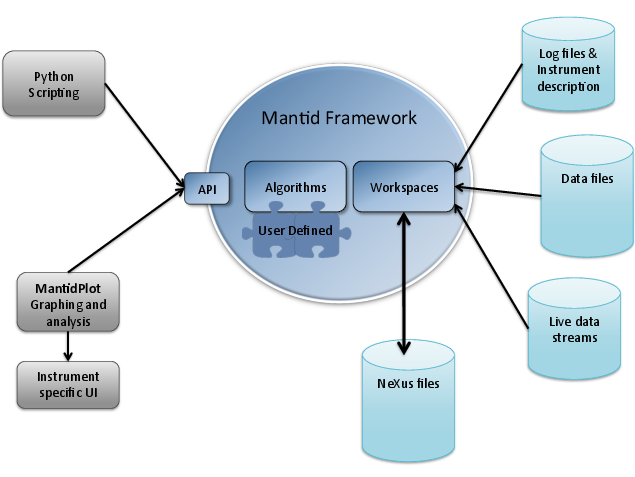
\includegraphics[width=0.75\textwidth]{MantidFramework.png}}
\caption{Mantid Framework design}
\label{fig:Framework}
\end{figure}

\subsection{Workspaces}
Workspaces are the data containers in Mantid. In addition to the data, workspaces can hold other types of information, such as instrument geometry, lattice parameters and orientation, or sample environment logs. Each workspace also holds its history, a list of algorithms that were used to create that workspace. That way each workspace can prove it's provenance, and also regenerate the commands used to make it. Depending on the organization of the data, there are various types and subtypes of workspaces.

Workspace2Ds contain data for multiple spectra, in the X, Signal, Error format, where X is a coordinate such as time of flight or energy transfer. The data acquisition system at several facilities now allow recording each  detected neutron, and labelling it with time-of-flight, and wall-clock-time stamps. For each spectrum, the EventWorkspace contains a list of events. EventWorkspaces can also provide a histogram representation as well,which is calculated on request. This allows event workspaces to support the MatrixWorkspace interface, also being supported by Workspace2Ds. The result is that algorithms and plotting work on the two types of workspaces interchangeably, without the need to know the details of how their data is stored. 
There are various uses for event workspaces. One can filter out unwanted events, such as events recorded during temperature spikes. The other big use for events is allowing novel techniques, such as asynchronous parameter scans (continuous angle scans, temperature scans), and pump probe experiments (pulse magnets, high frequency deformations of materials, and so on).

For data formats that contain different field types, Mantid provides various TableWorkspaces. A table workspace is organized in columns. Each column has a name and a type - the type of the data in that column. Examples of table workspaces are the outputs from the Fit algorithm, and PeaksWorkspaces, a representation of information about Bragg peaks, that is used in crystallography experiments.
 
The last major workspace type is the multi-dimensional workspace, or MDWorkspace. While for matrix workspace there are two dimensions describing a data point (spectrum number and X coordinate), for MDWorkspaces we have between 1 and 9 dimensions. For MDEventWorkspaces, each MDEvent contains coordinates, a weight and an error. It might contain also information about which detector and which run it come from. All MDEvents are contained in MDBoxes. Above a certain threshold, the MDBox becomes an MDGridBox, by splitting into several equal size MDBoxes. This allows for an efficient searching and binning, and allows plotting on an adaptive mesh. MDHistoWorkspaces consist of signal and error arrays on a regular grid.  

\subsection{Algorithms}
Mantid algorithms are procedures to manipulate workspaces. They can be predefined, or written by users, in either C++ or Python. At the present, there are over 500 algorithms in various categories, like data handling (loading/saving workspaces from/to files), arithmetic (plus, minus, multiply), unit conversions, and technique specific algorithms (powder diffraction, single crystal diffraction, SANS, reflectometry, direct and indirect spectrometry, and $\mu SR$). A particularly important set of algorithms was designed to deal with event data formats, to allow filtering and binning.

Algorithms can also be used to perform part of the work within other algorithms. This is particularly used within workflow algorithms, that specify a predefined series of steps to analyse particular data types within Mantid, starting with the raw files from the data acquisition system, and all intermediate stages, up to a format that scientists can work with.

Simple formatting, and input validation can transform user scripts in algorithms, and these can be shared with the entire Mantid community using the Mantid Script Repository, or by submitting them to the development team, to be included in the installation packages


\subsection{Python interface}
The most basic way to interact with the Mantid framework is through the python interface. By including the appropriate Mantid libraries, users can write their own reduction/analysis scripts, to execute their own custom reduction workflow. All algorithms are automatically exposed to python. In addition, several methods related to workspaces, and other helper objects are available as well. A tutorial of using the Python API can be found in the Documentation section on the Mantid webpage\cite{webpage}.  

Most reduction procedures for a particular instrument follow the same pattern, with minor parameter changes to account for experimental conditions. If there is enough metadata in the input files to get the required parameters, the Python interface allows the reduction process to occur automatically, as soon as the raw data file is saved. This is the case for several instruments at SNS. 

\subsection{MantidPlot}
For the average user, the main interaction with Mantid occurs through the MantidPlot interface (Figure \ref{fig:MantidPlot}). It is a graphical user interface based on QtiPlot\cite{qtiplot}. It allows simple 1D, and 2D plots of the data, and access to VATES interface for MDWorkspaces. Accessing the Python interface can be achieved through either the script window (run entire scripts at once) or the script interpreter (execute interactively single commands).

\begin{figure}[!ht]
\centerline{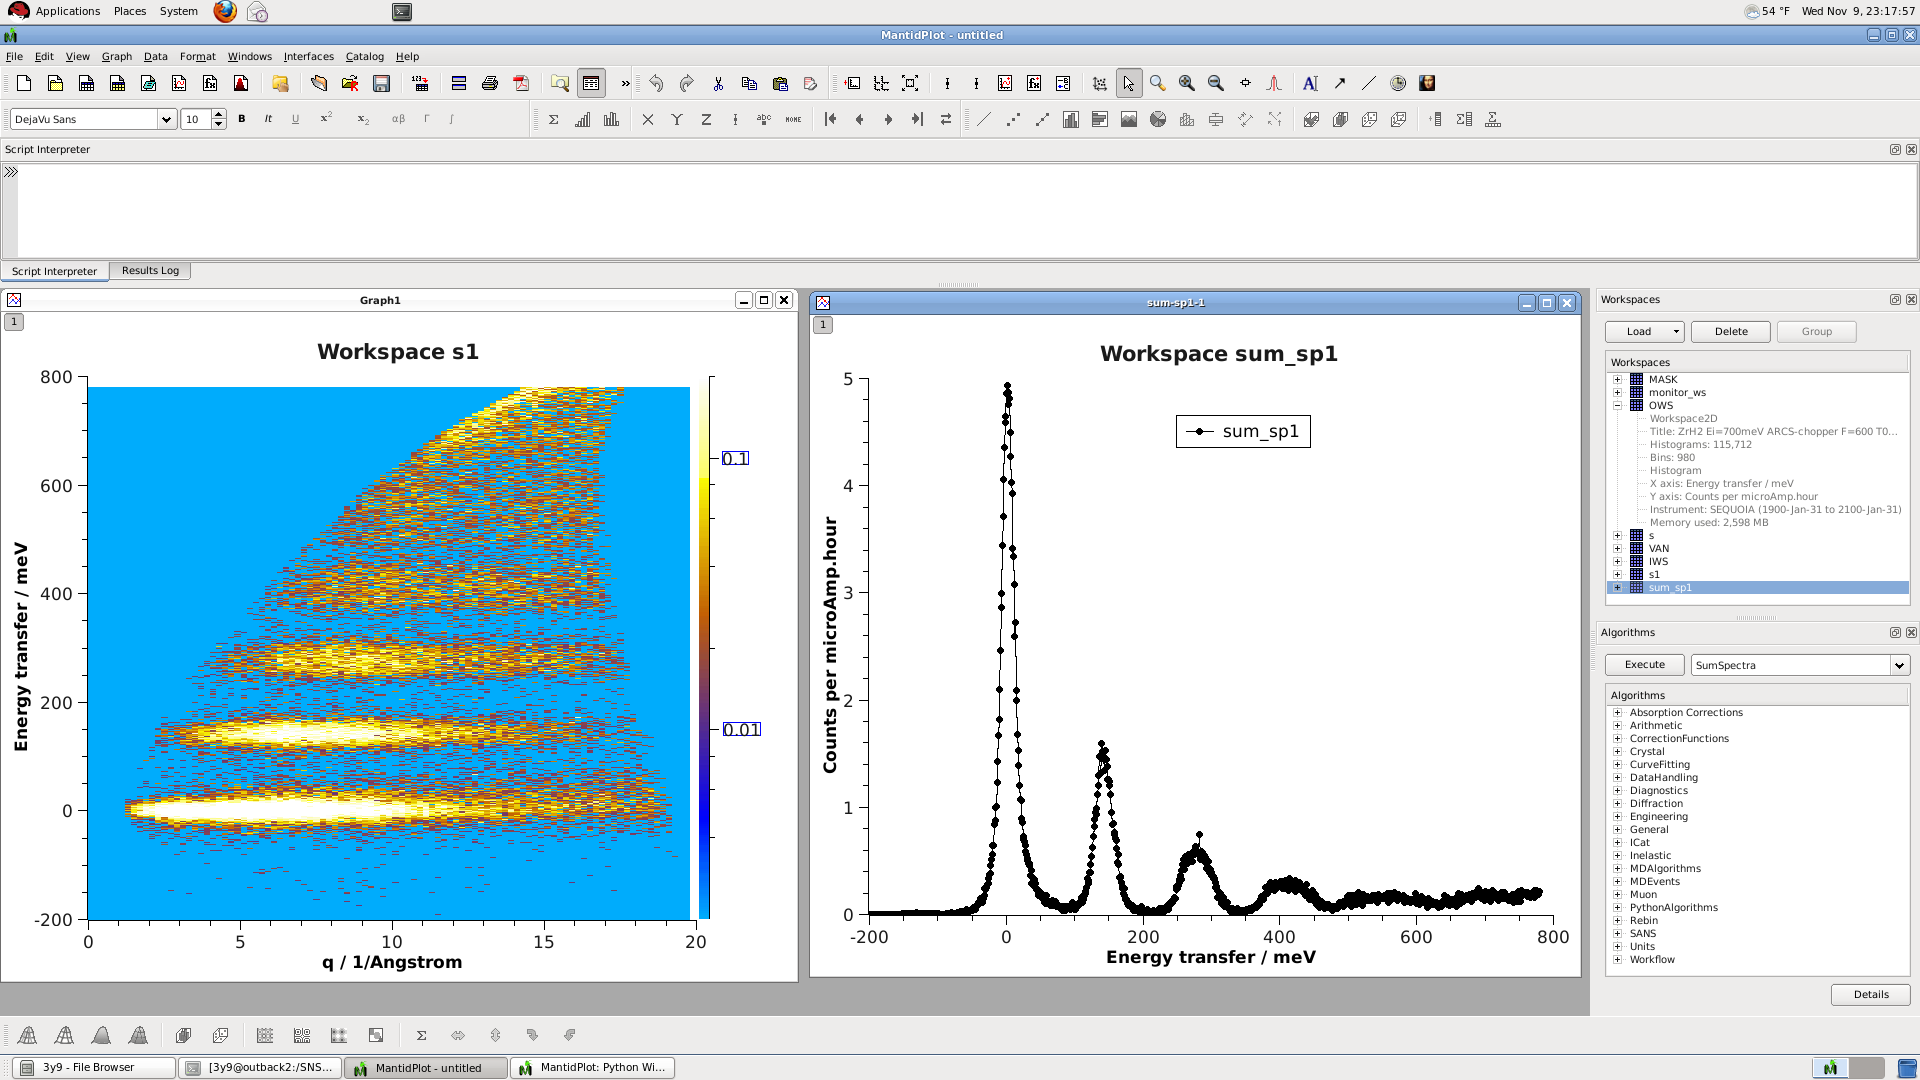
\includegraphics[width=0.75\textwidth]{MantidPlot.png}}
\caption{MantidPlot interface, showing 1D, and 2D plots. Lists of workspaces and algorithms are available on the right side}
\label{fig:MantidPlot}
\end{figure}
A list of available workspace is present by default. Clicking on the workspaces show information about workspace type and content. A context sensitive menu allows simple plotting, instrument view, inspection of the sample environment logs, or a listing of the history of the workspace.

A list of all algorithms is also present by default, organized both alphabetically, and by category. Clicking on an algorithm will open an automatically generated dialog box, with entries for each of the input parameters. A quick validation occurs when information is filled, and if any input is invalid it is going to be flagged. For each algorithm dialog box, a button allows for invoking the built-in help.

A results log window is also available, where users can see the results of running different algorithms.

For several scientific techniques, custom interfaces are available from the MantidPlot menu.



\subsection{Custom User Interfaces}
\begin{figure}[!ht]
\centerline{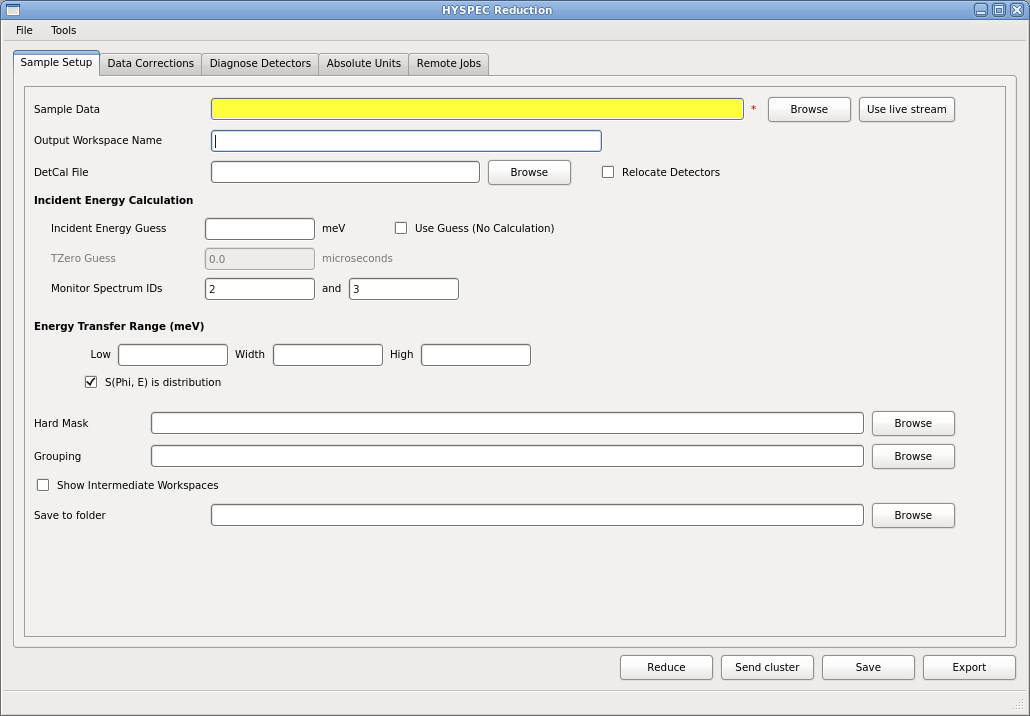
\includegraphics[width=0.75\textwidth]{Hyspec.png}}
\caption{Custom interface for direct geometry reduction on HYSPEC instrument}
\label{fig:Hyspec}
\end{figure}
Reduction scripts for several scientific techniques can be complicated, and depending on a large number of parameters. One can use either scripts of workflow algorithms to manipulate the raw data. The complexity of scripts can be intimidating for new users, while auto-generated dialog boxes for workflow algorithms can be unintuitive as well. Where needed, the development team has created custom user interfaces, to make complex analysis workflows much easier to use.

The custom user interfaces, available from MantidPlot, group together inputs from related reduction parameters, and spread independent steps onto different tabs. Figure \ref{fig:Hyspec}, shows an example, the DGS Reduction interface for the HYSPEC instrument at SNS. When it is executed on computers with certain privileges, advanced option can appear or disappear, like live data analysis, or sending reduction jobs to particular computing clusters.
Other interfaces exist for data reduction and analysis for various techniques, including $\mu SR$\cite{musr}, small angle neutron scattering, indirect spectroscopy, single crystal diffraction, and reflectometry.

\subsection{VATES}
\begin{figure}[ht]
\centerline{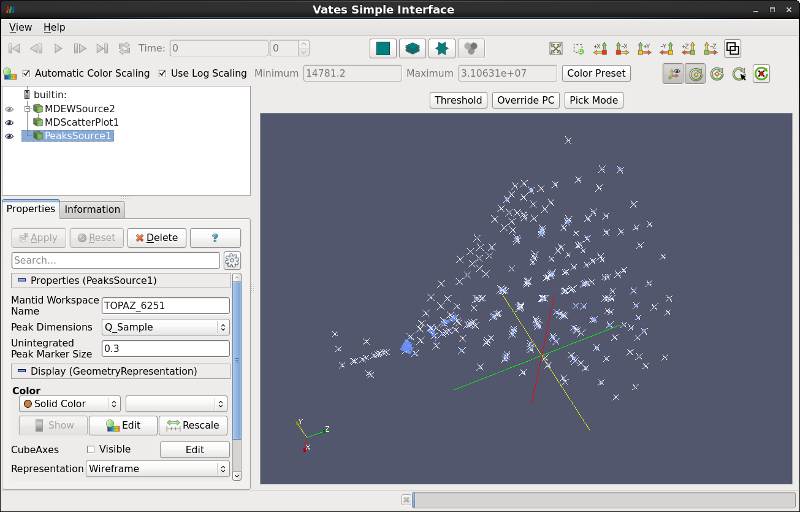
\includegraphics[width=0.75\textwidth]{VSI-v2-SplatterPlot.png}}
\caption{VSI in splatter plot mode with single crystal data from TOPAZ difractometer.}
\label{fig:VSI_sample}
\end{figure}
For visualizing 3 and 4 dimension datasets, Mantid provides the VATES Simple Interface (\textit{VSI}), that offers a stock set of data views and access to a subset of Mantid algorithms. It is based on application widgets and rendering libraries from the ParaView\cite{paraview} visualization program. The \textit{VSI}$\*$ takes advantage of the ParaView plugin architecture to provide functionality from within Mantid and from within ParaView standalone. The data in Mantid to be visualized passes through an API layer which translates the internal Mantid data structure to a VTK\cite{vtk} data structure, that can be rendered in the \textit{VSI}$\*$. Those same data structures can be saved to file and visualized in the ParaView program. The API layer provides the desired decoupling of the data structures and provides good flexibility to handle the various needs of the Mantid data structures and algorithms. 

\begin{figure}[!hb]
\centerline{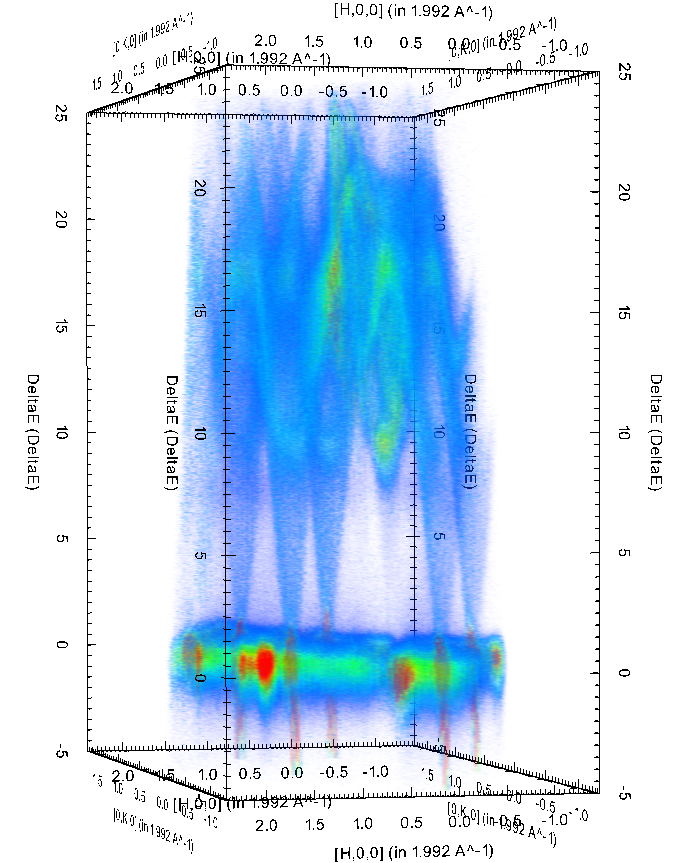
\includegraphics[width=0.6\textwidth]{NonOrthogonalProjection_W.png}}
\caption{Volume rendering of Gd excitations, in ParaView. Data was measured on SEQUOIA spectrometer at SNS.}
\label{fig:ParaView_sample}
\end{figure}

The \textit{VSI}$\*$ has a view called MultiSlice which allows placing multiple orthogonal slices on the data. Those slices can then alternately be viewed in SliceViewer. The SplatterPlot (Figure 1) view is oriented towards visualizing peaks in single crystal diffraction data. In that view, there is a pick mode which can interact with Mantid to retrieve information about a selected peak. The ThreeSlice view shows three orthogonal planes through the data with the capability exploring via moving a crosshair in one of the planes with a coordinate readout in each plane to show the location. The \textit{VSI}$\*$ has the ability to show the data with non-orthogonal axes such as the data in Figure 2. This capability was implemented by Kitware\cite{kitware} via the SNS in support of the Mantid project.






\section{Conclusion}
The Mantid project offers an extensible framework for data manipulation, analysis and visualization, geared toward neutron scattering and $\mu SR$ experiments. It is the main reduction software in use at SNS and ISIS, and partially in use or considered at several other scientific facilities. Up to date information, and usage tutorials can be found on the Mantid web page\cite{webpage}. 

The development team would like to thank various instrument scientists for their feedback. Work at ORNL was sponsored by the Scientific User Facilities Division, Office of Basic Energy Sciences, US Department of Energy. 


% The Appendices part is started with the command \appendix;
% appendix sections are then done as normal sections
% \appendix

% \section{}
% \label{}

\begin{thebibliography}{00}
\bibitem{Egami} Takeshi Egami and Simon J.L. Billinge, Editor(s), Pergamon Materials Series, Pergamon, 2003, Volume 7
\bibitem{Nojiri} H. Nojiri {\it et al.}, Phys. Rev. Lett. 106, 237202 (2011)
\bibitem{Wang} X.L. Wang {\it et al.}, Scientific Reports 2, 747 (2012)
\bibitem{DAVE}  R.T. Azuah {\it et al.}, J. Res. Natl. Inst. Stan. Technol. 114, 341 (2009).
\bibitem{OpenGenie} S.I. Campbell {\it et al.}, arXiv:cond-mat/0210442
\bibitem{LAMP} D. Richard, M. Ferrand and G.J. Kearley, J. Neutron Research 4, 33-39, 1996
\bibitem{ISAW} ISAW
\bibitem{trac} trac
\bibitem{github} github
\bibitem{jenkins} jenkins
\bibitem{webpage} http://www.mantidproject.org
\bibitem{qtiplot} http://soft.proindependent.com/qtiplot.html
\bibitem{musr} S. Cottrell {\it et. al.}, Physics Procedia 30, 20-25 (2012)
\bibitem{paraview} A. Henderson, ParaView Guide, A Parallel Visualization Application, Kitware Inc.(2007)
\bibitem{vtk} W. Schroeder {\it et. al.}, The Visualization Toolkit, Kitware Inc.(2006)
\bibitem{kitware} http://www.kitware.com

\end{thebibliography}

\end{document}


